\documentclass[conference]{IEEEtran}
\usepackage{graphicx}
\usepackage{booktabs}
\usepackage{amsmath}
\usepackage{hyperref}

\title{Pulmonary Nodule False Positive Reduction from CT Images Using 3D CNN on the LUNA16 Dataset}
\author{Lab Report}

\begin{document}

\maketitle

\begin{abstract}
We apply a 3D CNN to the false positive reduction task on the LUNA16 dataset, classifying $32^3$-voxel patches centered on candidate locations as nodule or non-nodule. Using Focal Loss and balanced sampling to handle extreme class imbalance (${\sim}1{:}484$), the model achieves an AUC-ROC of 0.9978, sensitivity of 0.9941, and specificity of 0.9616.
\end{abstract}

\section{Introduction}
Pulmonary nodules are small lung masses that may indicate early-stage lung cancer. Automated CAD systems can improve CT screening efficiency but typically produce many false positives. The LUNA16 challenge~\cite{setio2017validation} addresses this through a false positive reduction track: classifying pre-computed candidate locations as true nodules or false positives. We tackle this task using a 3D CNN and evaluate with standard classification metrics (AUC-ROC, sensitivity, specificity, F1).

\section{Exploratory Data Analysis}

The LUNA16 dataset contains 888 CT scans with annotations from four radiologists. We use subsets 0--4 (445 scans) available on Kaggle. Table~\ref{tab:stats} summarizes key statistics; the \texttt{candidates\_V2.csv} file provides 754,975 candidate locations with a ${\sim}1{:}484$ class imbalance (Fig.~\ref{fig:eda_class}). Nodule diameters are right-skewed (median 6.4~mm, mean 8.3~mm). CT scans have typical axial resolution of $512 \times 512$ with 0.7~mm in-plane spacing and 0.625--2.5~mm slice thickness.

\begin{table}[h]
\centering
\caption{LUNA16 Dataset Statistics}
\label{tab:stats}
\begin{tabular}{@{}lr@{}}
\toprule
Metric & Value \\ \midrule
CT scans (available subsets 0--4) & 445 \\
Annotated nodules (available) & 615 \\
Candidates V2 (total) & 754,975 \\
Positive / Negative candidates & 1,557 / 753,418 \\
Class imbalance ratio & $\sim$1:484 \\
Nodule diameter mean / median & 8.3 / 6.4~mm \\
\bottomrule
\end{tabular}
\end{table}

\begin{figure}[h]
    \centering
    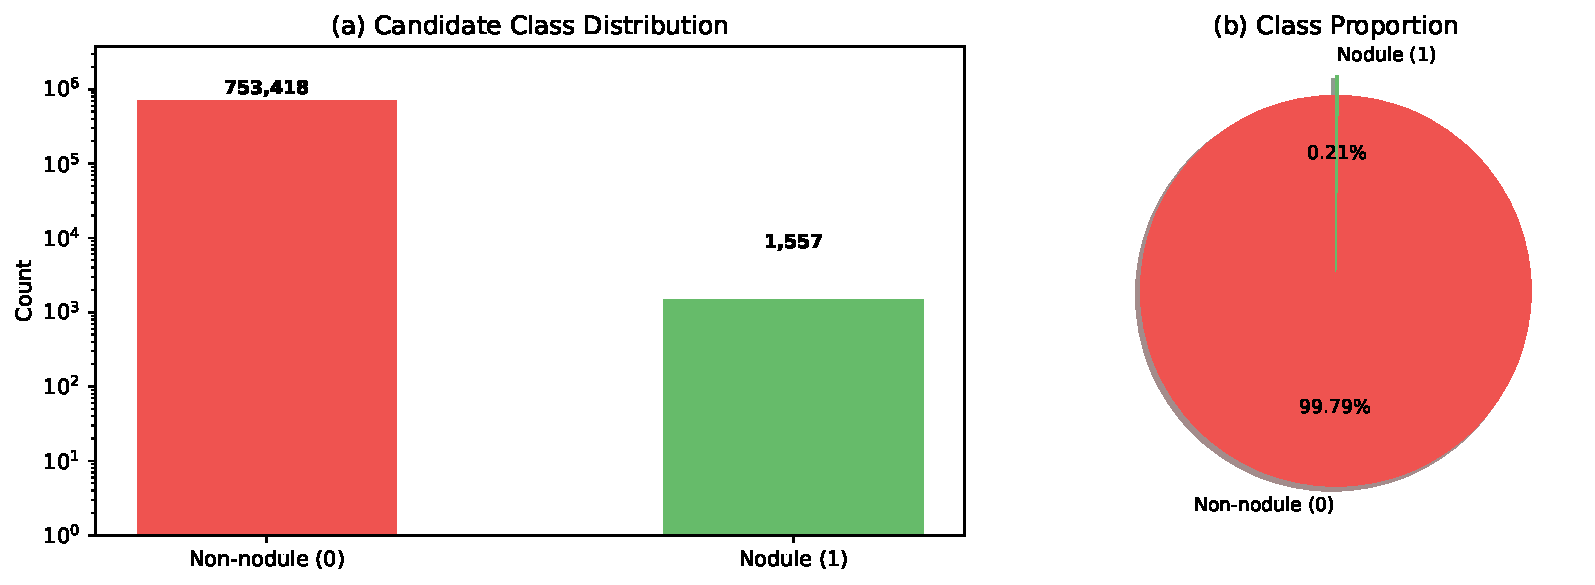
\includegraphics[width=\columnwidth]{fig/candidate_class_distribution.pdf}
    \caption{Candidate class distribution showing extreme imbalance (${\sim}1{:}484$). (a)~Log-scale bar chart. (b)~Proportion.}
    \label{fig:eda_class}
\end{figure}

Fig.~\ref{fig:patches} illustrates the visual similarity between nodule and non-nodule patches that makes classification challenging.

\begin{figure}[h]
    \centering
    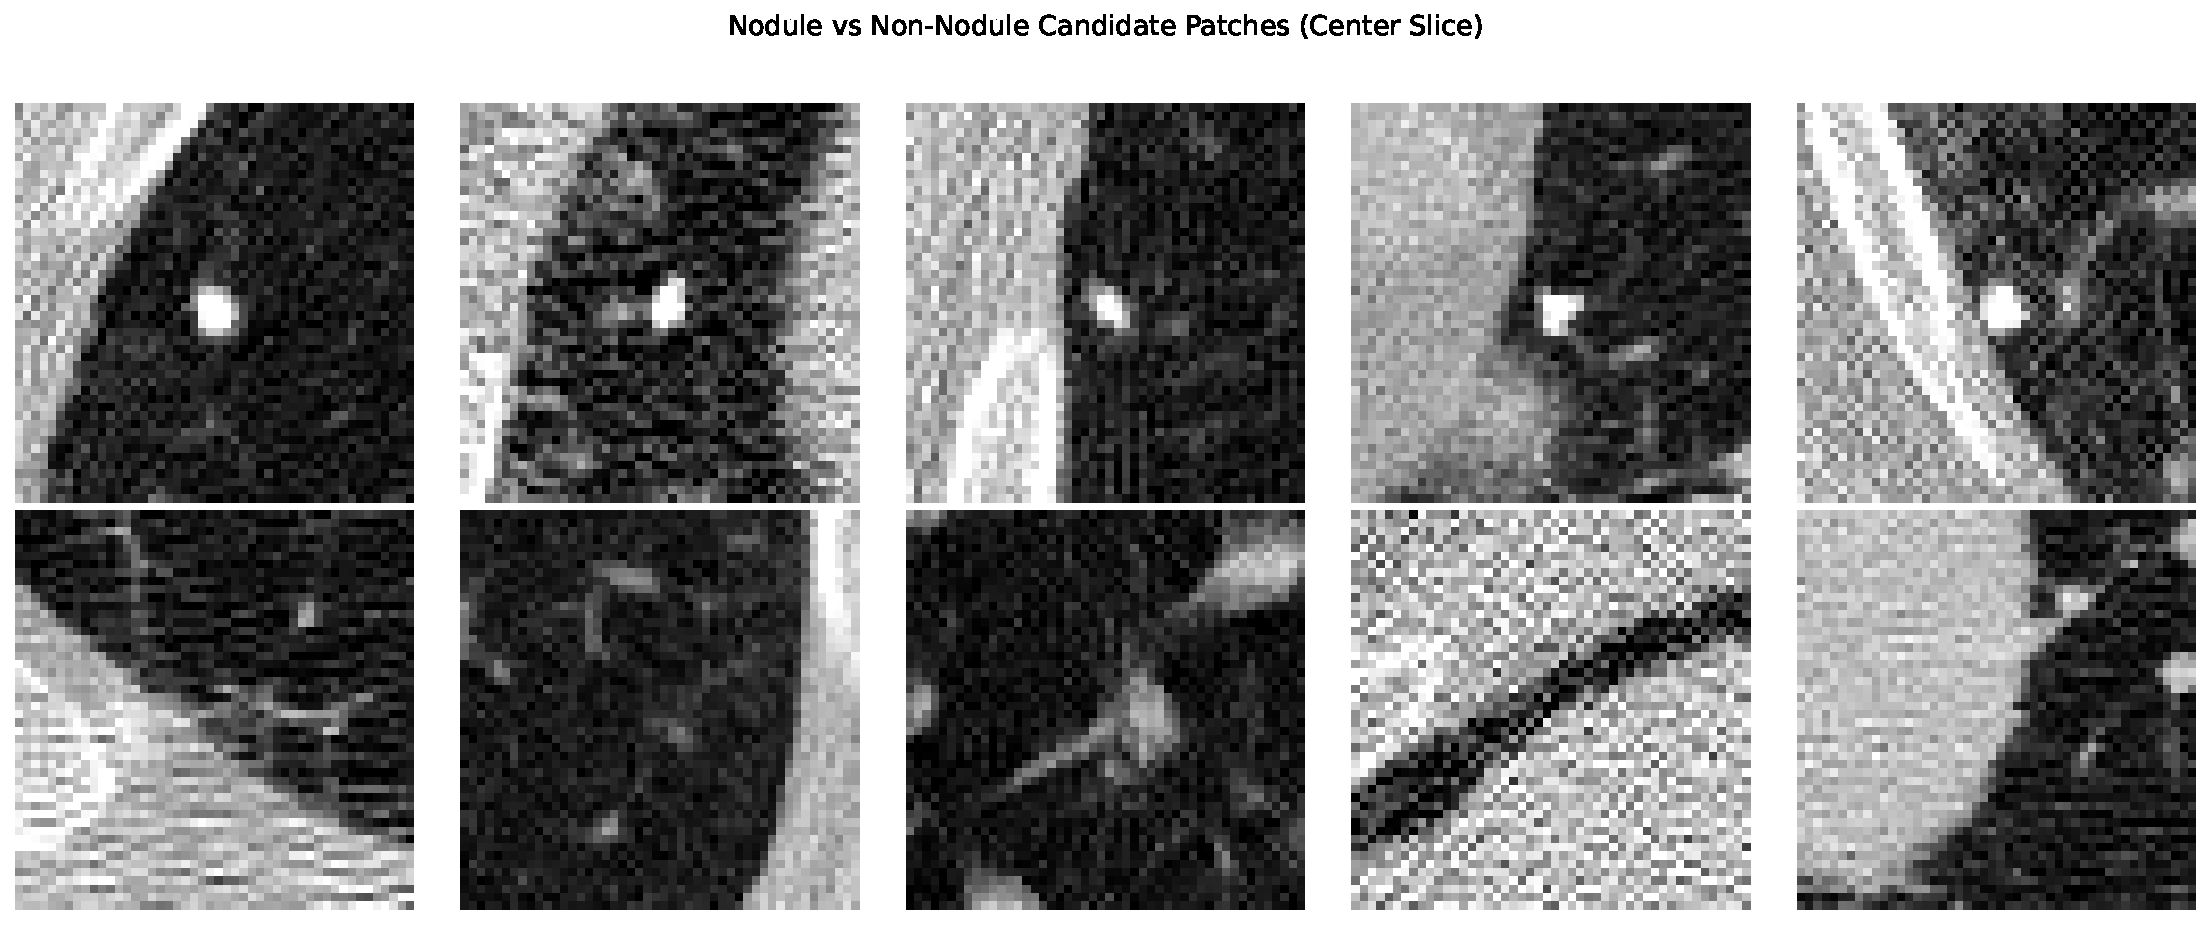
\includegraphics[width=0.9\columnwidth]{fig/nodule_vs_nonnodule_patches.pdf}
    \caption{Nodule (top) vs non-nodule (bottom) candidate patches. Center axial slices shown.}
    \label{fig:patches}
\end{figure}

\section{Methods}

\subsection{Data Pipeline and Augmentation}
For each candidate, we load the CT scan via SimpleITK, convert world coordinates to voxel indices, extract a $32^3$ patch (zero-padded at boundaries), and normalize HU values from $[-1000, 400]$ to $[0, 1]$. To address memory constraints, negative candidates are subsampled to a 1:20 ratio, reducing ${\sim}377$K to ${\sim}16$K total patches. Subsets 0--3 are used for training and subset~4 for validation. A \texttt{WeightedRandomSampler} ensures balanced 1:1 training epochs. Augmentation includes random 3D flips (50\%), 90$^\circ$ axial rotations, and Gaussian noise ($\sigma = 0.01$, 50\%).

\subsection{3D CNN Architecture}
The model (${\sim}7.0$M parameters) has four convolutional blocks followed by a three-layer classifier:
\begin{itemize}
    \item \textbf{Blocks 1--3}: Conv3d $\times 2$ + BN + ReLU + MaxPool($2^3$), channels $1 \to 64 \to 128 \to 256$
    \item \textbf{Block 4}: Conv3d($256 \to 512$) + BN + ReLU + GlobalAvgPool
    \item \textbf{Classifier}: FC($512 \to 128$) + Drop(0.5) $\to$ FC($128 \to 64$) + Drop(0.3) $\to$ FC($64 \to 1$)
\end{itemize}

\subsection{Training and Evaluation}
We use Focal Loss ($\alpha{=}0.75$, $\gamma{=}2.0$) with Adam (lr $= 10^{-3}$, wd $= 10^{-4}$), ReduceLROnPlateau scheduler, mixed-precision training on an NVIDIA P100, batch size 32, and early stopping (patience 8 on val AUC). Evaluation metrics include AUC-ROC, and sensitivity/specificity/F1 at the optimal Youden's J threshold ($J = \text{TPR} - \text{FPR}$).

\section{Results}

Table~\ref{tab:results} summarizes the validation performance. The model achieves AUC-ROC of 0.9978, indicating near-perfect candidate-level discrimination. At the optimal threshold, sensitivity is 99.41\% with 96.16\% specificity. The confusion matrix (Fig.~\ref{fig:cm}) shows most errors are false positives.

\begin{table}[h]
\centering
\caption{Validation Results (Subset 4)}
\label{tab:results}
\begin{tabular}{@{}lc@{}}
\toprule
Metric & Value \\ \midrule
AUC-ROC & \textbf{0.9978} \\
Sensitivity & 0.9941 \\
Specificity & 0.9616 \\
F1-Score & 0.7226 \\
\bottomrule
\end{tabular}
\end{table}

\begin{figure}[h]
    \centering
    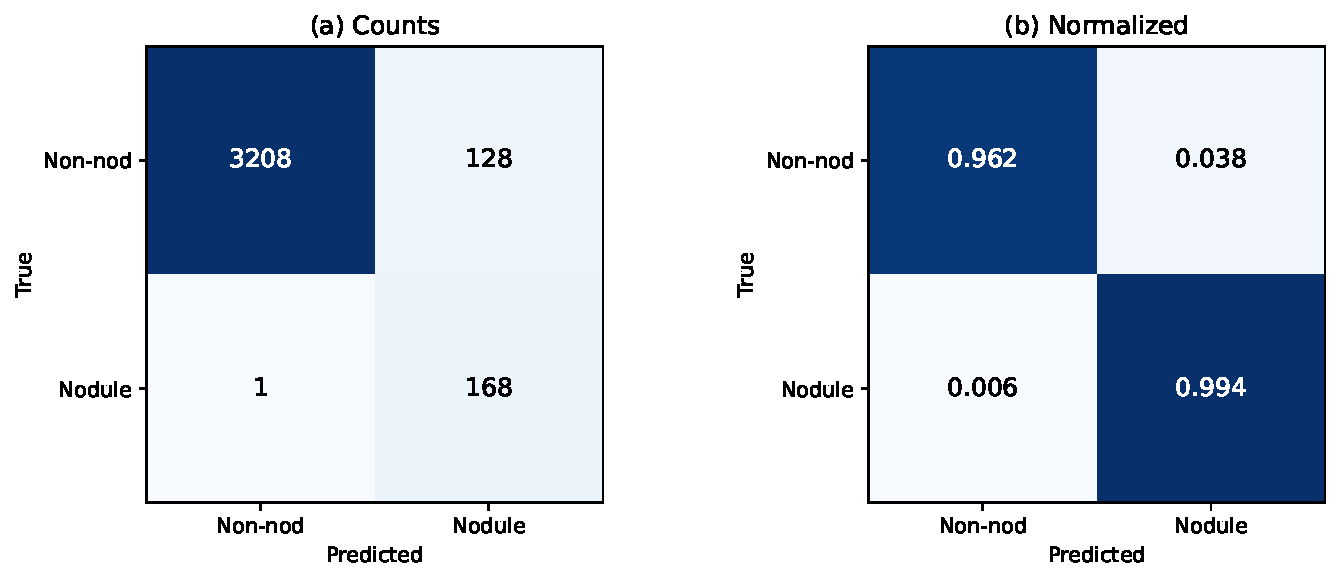
\includegraphics[width=\columnwidth]{fig/confusion_matrix.pdf}
    \caption{Confusion matrix: (a)~raw counts, (b)~row-normalized.}
    \label{fig:cm}
\end{figure}



\subsection{Qualitative Results}
Fig.~\ref{fig:preds} shows sample predictions. The model correctly identifies most nodules with high confidence while assigning low probabilities to non-nodule candidates.

\begin{figure}[h]
    \centering
    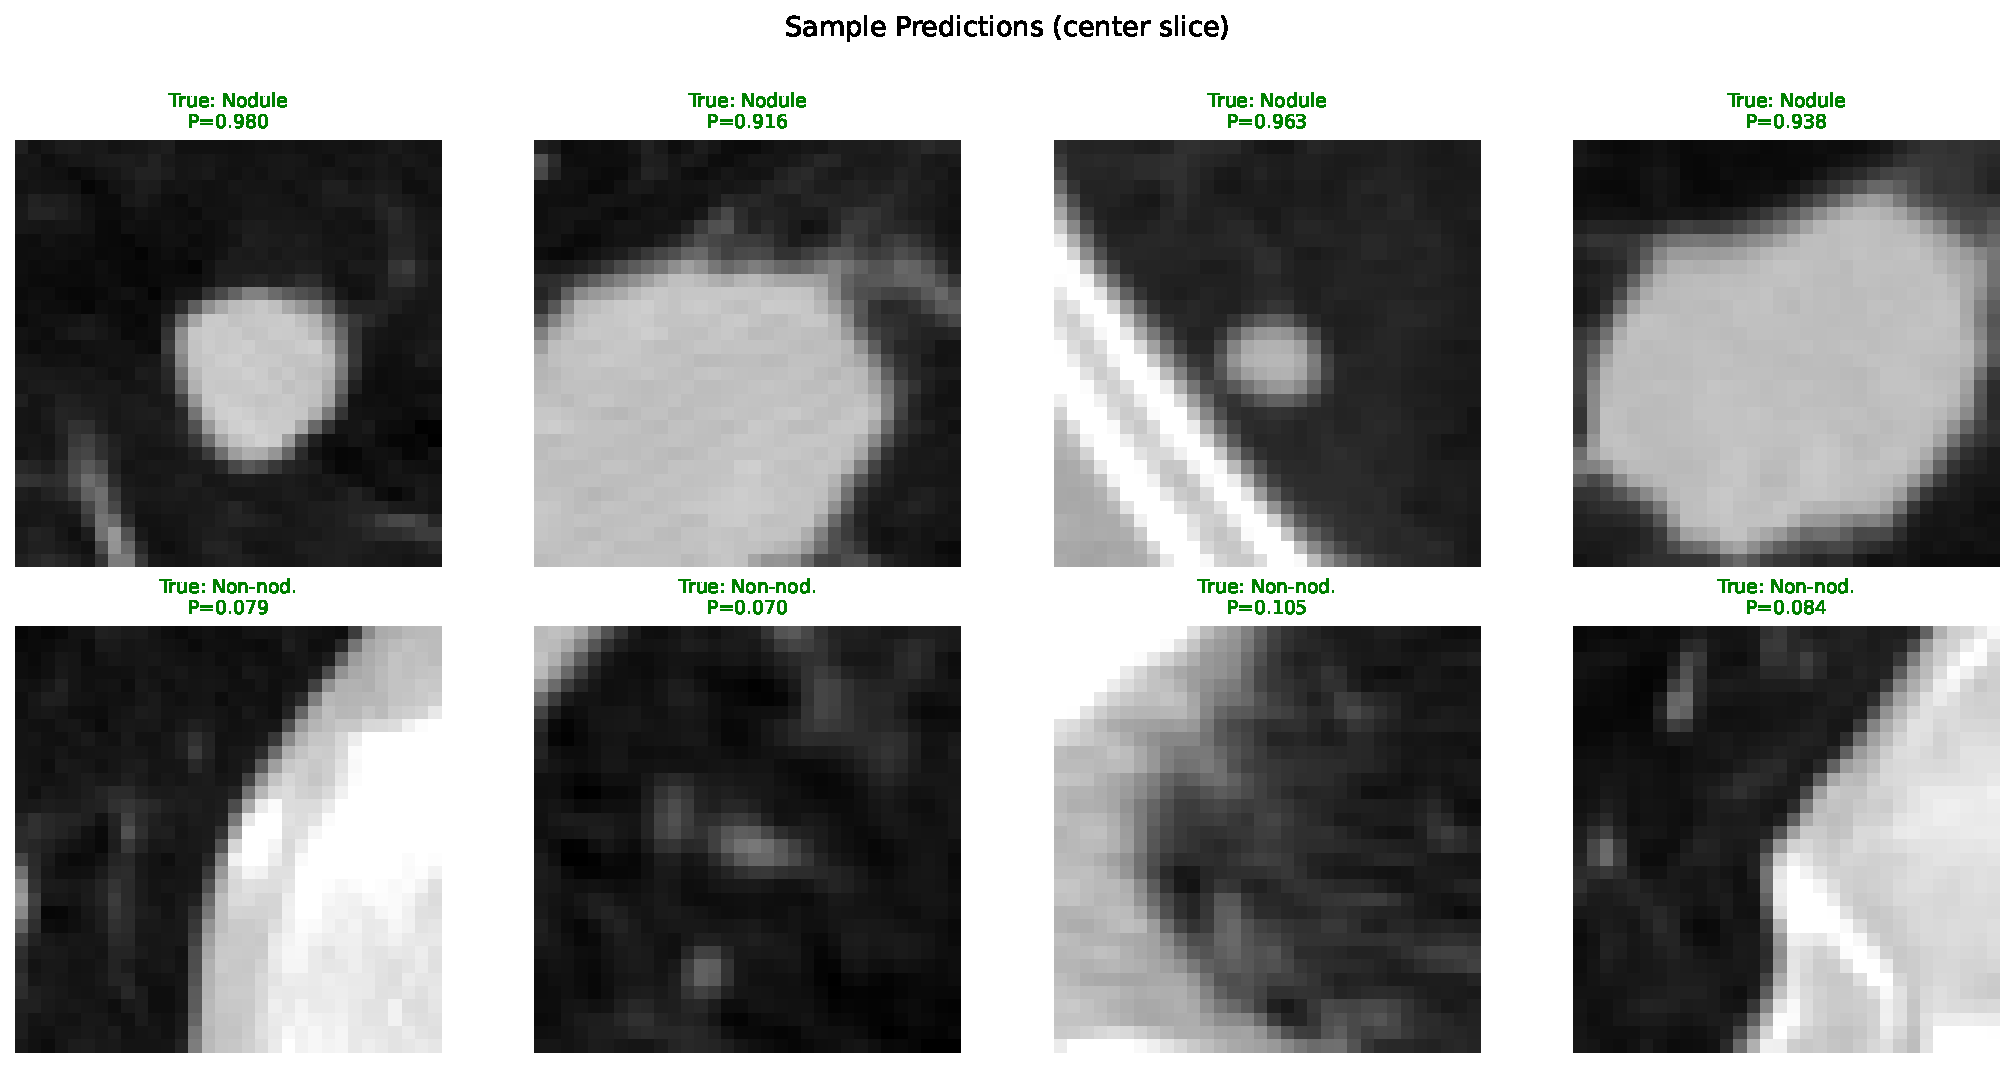
\includegraphics[width=0.9\columnwidth]{fig/sample_predictions.pdf}
    \caption{Sample predictions. Top: true nodules; bottom: true non-nodules. Green = correct, red = incorrect.}
    \label{fig:preds}
\end{figure}

\section{Discussion}

\textbf{Class imbalance handling.} Focal Loss ($\gamma{=}2.0$) combined with balanced sampling effectively addresses the ${\sim}1{:}484$ imbalance by down-weighting easy negatives.

\textbf{Limitations.} Only subsets 0--4 are used (half the data), and memory-constrained subsampling limits hard negative diversity. Future work could explore 3D ResNets, attention mechanisms, larger patches, and evaluation on the full dataset.

\section{Conclusion}
A 3D CNN with Focal Loss and balanced sampling achieves AUC-ROC of 0.9978 with 99.41\% sensitivity and 96.16\% specificity on the LUNA16 false positive reduction task. Training on the full dataset with deeper architectures could further improve performance.

\begin{thebibliography}{1}
\bibitem{setio2017validation}
A.~A.~A.~Setio \textit{et al.}, ``Validation, comparison, and combination of algorithms for automatic detection of pulmonary nodules in computed tomography images: The LUNA16 challenge,'' \textit{Medical Image Analysis}, vol.~42, pp.~1--13, 2017.
\end{thebibliography}

\end{document}
